\section{Introduction}
\begin{frame}
	\frametitle{Introduction}
	We can derive the mathematical model of a dynamic system in two ways mainly:
	\begin{itemize}
		\item Physical Modeling: 
		
		Applying the laws of physics, chemistry, thermodynamics,...
		Also called modeling from \emph{First Principles}
		
		\pause 
		
		\item  System identification or \emph{Empirical Modeling}:
		
		Developing models from observed or collected data
		\begin{figure}
			\centering
			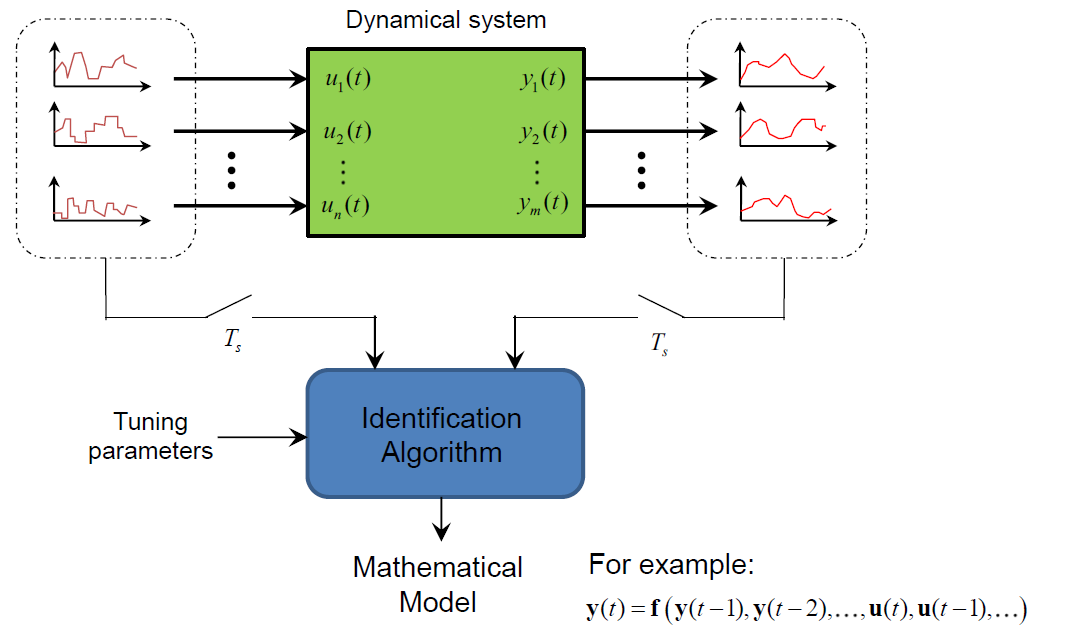
\includegraphics[width=0.7\linewidth]{img/system-identification}
			%\caption{}
			\label{fig:system-identification}
		\end{figure}
		
	\end{itemize}
\end{frame}


\section{First Principles Modeling}

% Counter for the example numbers
\newcounter{exampleCount}

\begin{frame}
	\stepcounter{exampleCount}
	\frametitle{Example \arabic{exampleCount}: Mass-Spring System} 
	
	\begin{columns}
		\begin{column}{0.4\linewidth}
			\begin{figure}
				\centering
				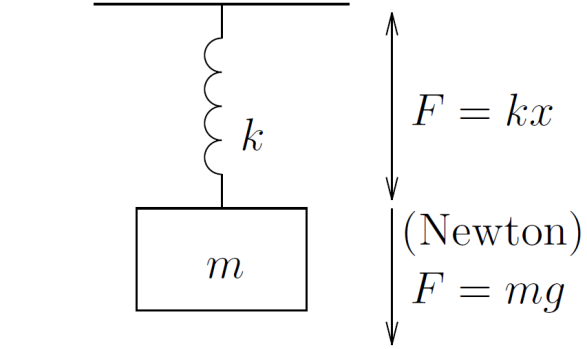
\includegraphics[width=1\linewidth]{img/mass-spring}
				\label{fig:mass-spring}
			\end{figure}
		\end{column}
		\begin{column}{0.6\linewidth}
			If spring is at rest at $x=0$:
			\begin{align*}
			m \cdot \frac{d^{2}x}{dt^{2}} + k \cdot x =  m \cdot g \\
			\end{align*}
		\end{column}
	\end{columns}
\end{frame}


\begin{frame}
	\stepcounter{exampleCount}
	\frametitle{Example \arabic{exampleCount}: Mass-Spring Damped}
	\begin{figure}
		\centering
		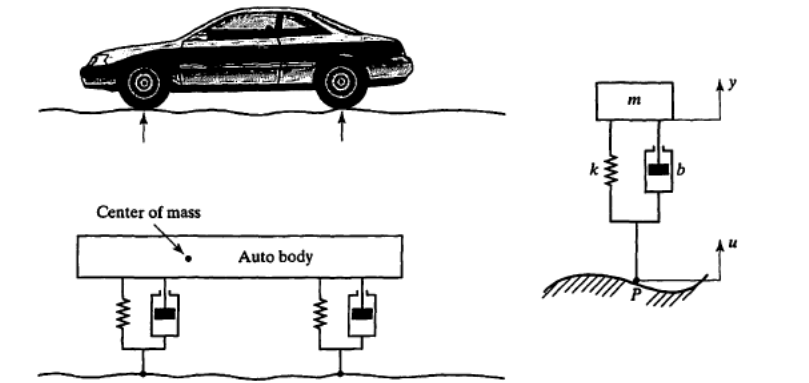
\includegraphics[width=1\linewidth]{img/mass-spring-damped}
		\label{fig:mass-spring-damped}
	\end{figure}
	Force excerted by damper: $F = b\dot{x}$
	
	Differential equation can be found by writing force equilibrium and moment equilibrium around center of mass
	
	%\emph{\textcolor{blue}{ \href{https://youtu.be/8DuJEpy-ODo}{Animation} }}
\end{frame}

\begin{frame}
	\stepcounter{exampleCount}
	\frametitle{Example \arabic{exampleCount}: Pendulum}
	\begin{columns}
		\begin{column}{0.4\linewidth}
			\begin{figure}
				\centering
				\includegraphics[width=1\linewidth]{img/new-pendulum}
				\label{fig:pendulum}
			\end{figure}
		\end{column}
		\begin{column}{0.6\linewidth}
			Dynamic equilibrium:
			\begin{align*}
			&I\ddot{\theta}(t) = -m g \frac{L}{2} \sin(\theta(t)) \text{ with } I= \frac{m L^2}{3} \\
			&\ddot{\theta}(t)  = -\frac{3g}{2L} \sin(\theta(t)) 
			\end{align*}
			
			Small deviation of $\theta(t)$: \\
			\hspace{1cm} $\ddot{\theta}(t) = -\frac{3g}{2L} \theta(t)$
			
			Solving the differential equation yields the general solution:
			$\theta(t) = A\cos(\omega_0 + \phi)$
			with $\omega_0=\sqrt{\frac{3g}{2L}}$ and $\phi$ \& $A$ to be determined with the initial condition
		\end{column}
	\end{columns}
\end{frame}

\begin{frame}
	\stepcounter{exampleCount}
	\frametitle{Example \arabic{exampleCount}: Inverted Pendulum}
	\begin{columns}
		\begin{column}{0.6\linewidth}
			\begin{figure}
				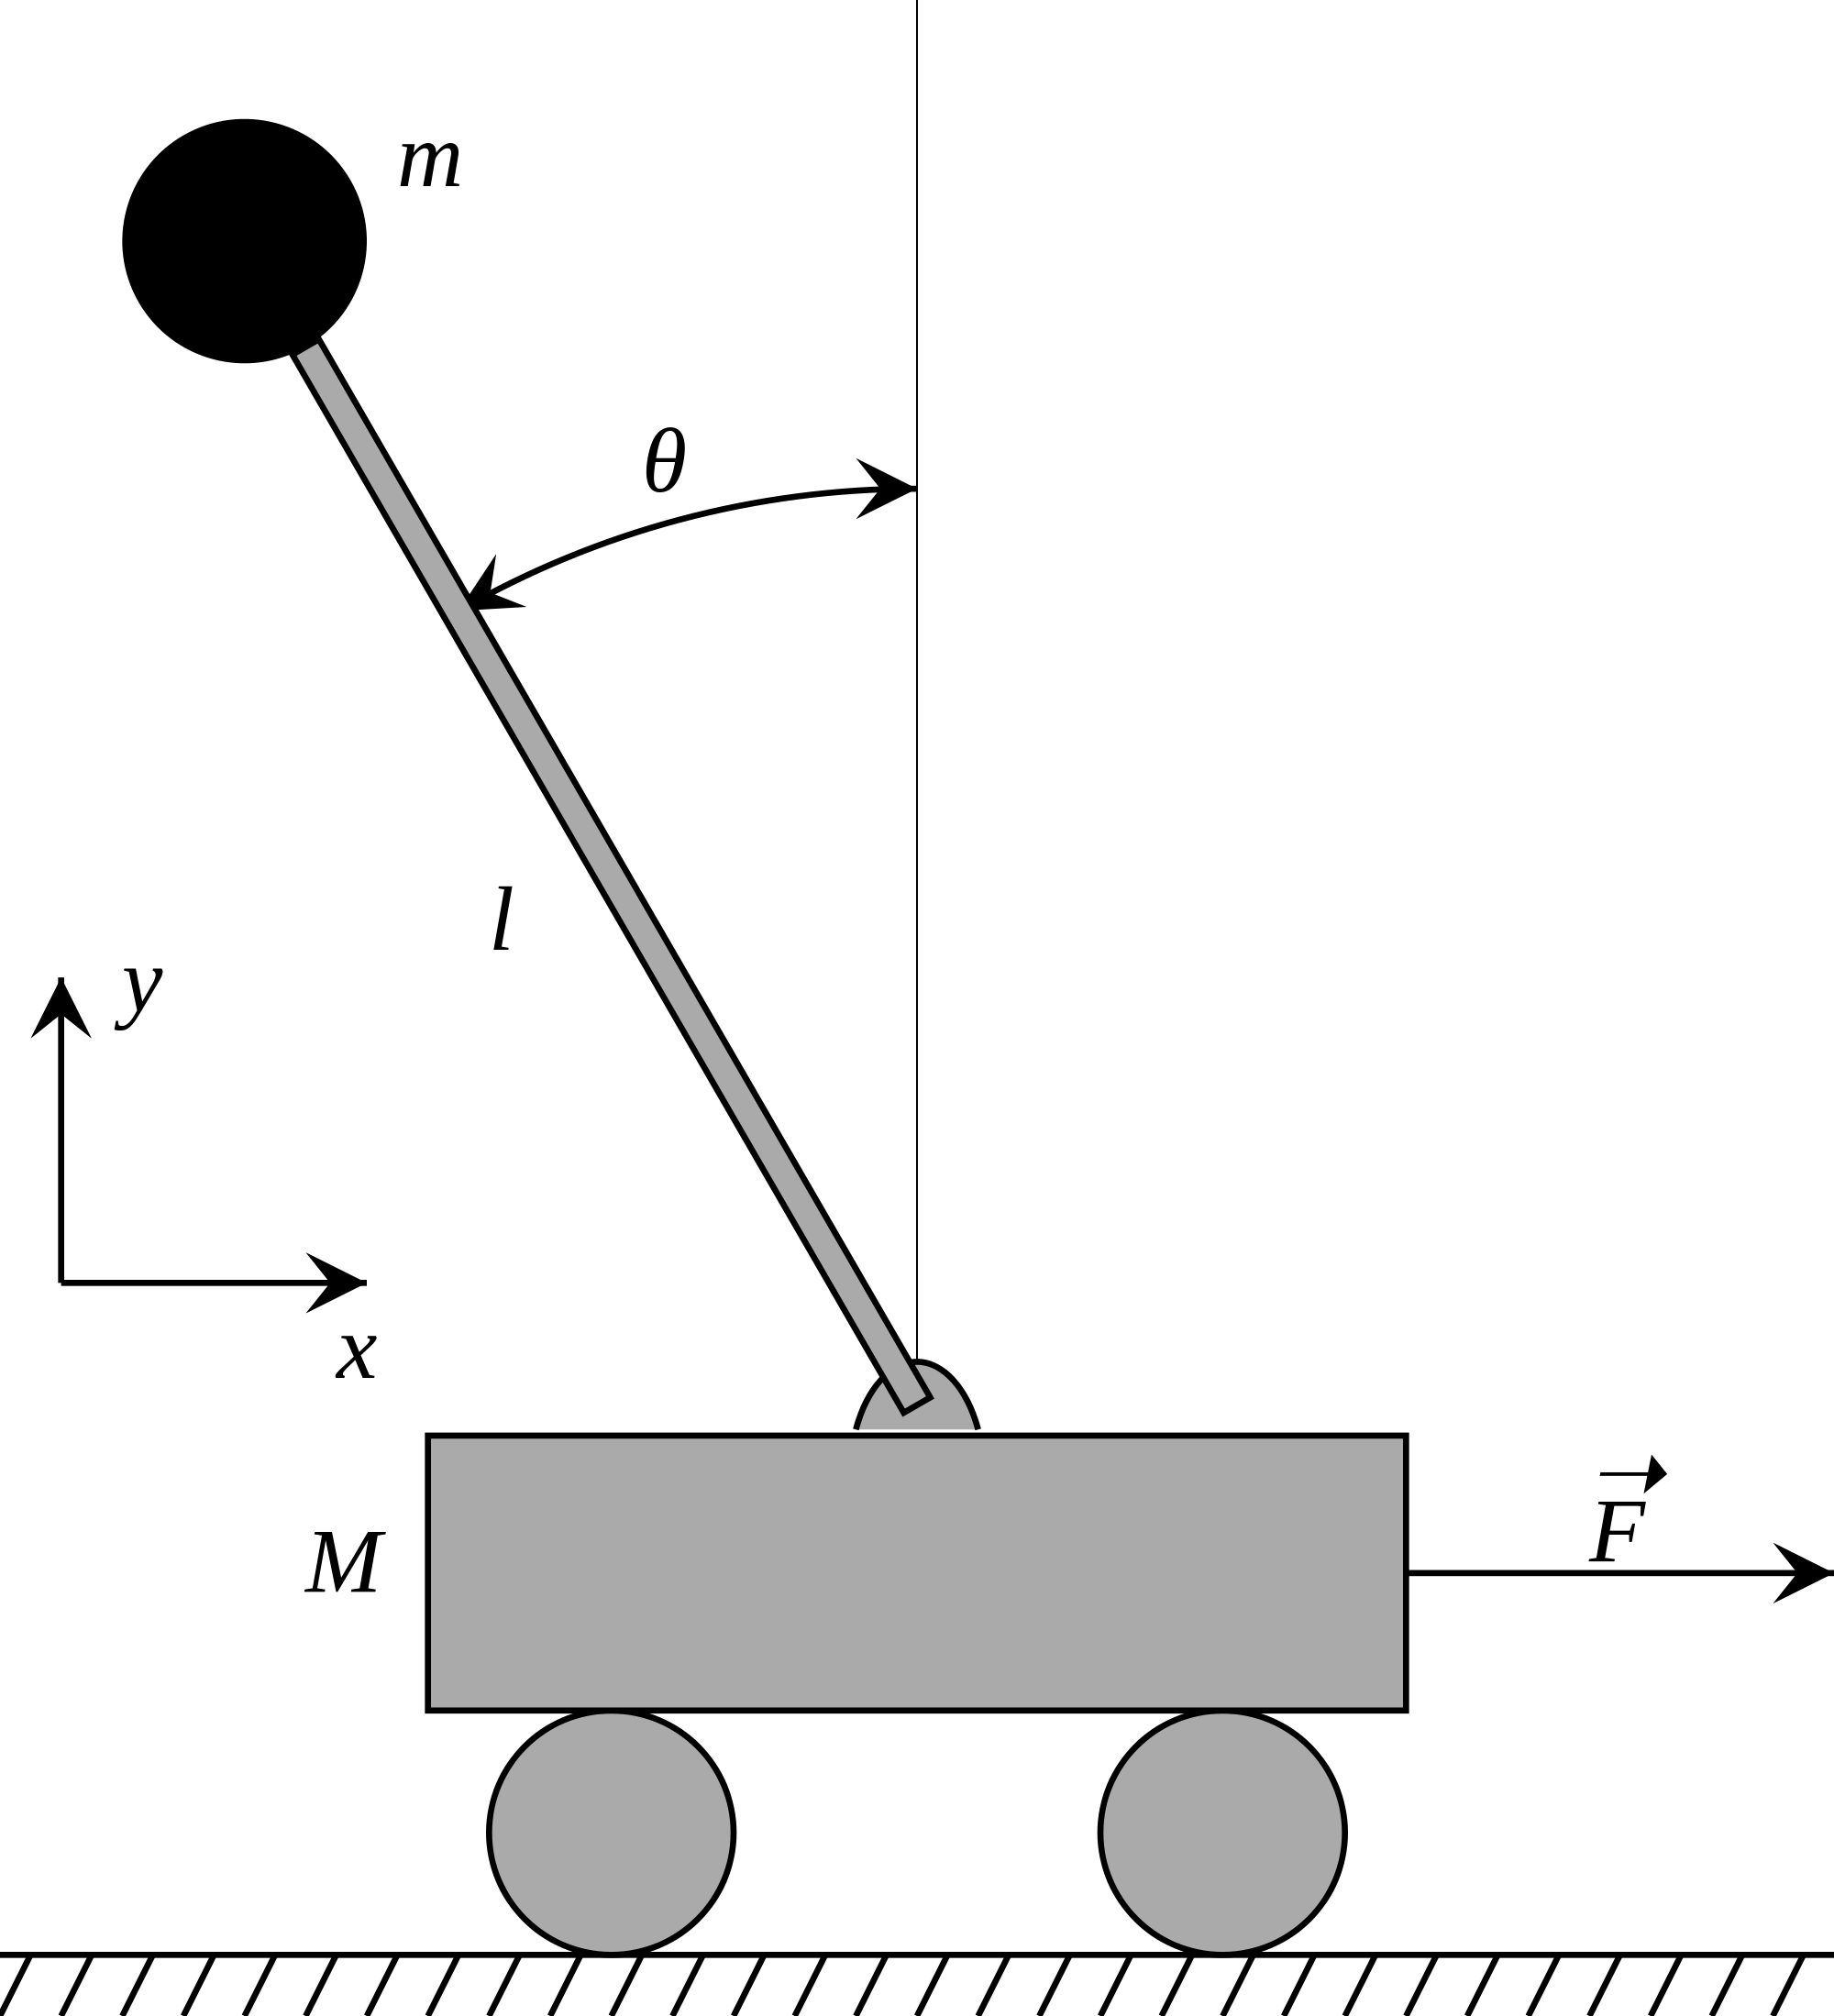
\includegraphics[width=1\linewidth]{img/pendulum-inverted}
				\label{fig:pendulum-inverted}
				%youtube: https://www.youtube.com/watch?v=15DIidigArA
			\end{figure}
		\end{column}
		\begin{column}{0.4\linewidth}
			Analysis can be done with Newton like former example, but less tedious is using energy-methods (Lagrange)
			
		\end{column}
	\end{columns}
	
\end{frame}

\begin{frame}
	\stepcounter{exampleCount}
	\frametitle{Example \arabic{exampleCount}: RLC Circuit}
	
	\begin{figure}
		\centering
		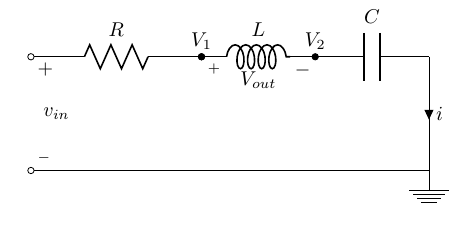
\includegraphics[width=0.7\linewidth]{img/circuit-RLC}
		\label{fig:circuit-RLC}
	\end{figure}
	Besides input $v_{in}$, two internal variables are needed to determine output $\Rightarrow$ Second-order System
	\begin{center}
		\begin{tabular}{c@{\hskip 1cm} c@{\hskip 1cm} c}
			Inputs 	& Ouputs 	& Choosen States \\ \hline
			$v_{in}$ 	& $v_{out}$	& $V_2$ \\
			& & $i$ \\ 
		\end{tabular}
	\end{center}
	
\end{frame}

\begin{frame}
	
	\frametitle{Example \arabic{exampleCount}: RLC Circuit}
	
	\begin{columns}
		\begin{column}{0.4\linewidth}
			Equations for each component:
			\begin{align*}
			&i = \frac{V_{in} - V_{1}}{R} \\
			&V_1 - V_2 = L \cdot \frac{di}{dt} \\
			&i = C \cdot \frac{dV_2}{dt} \\
			\end{align*}
		\end{column}
		\begin{column}{0.6\linewidth}
			\begin{figure}
				\centering
				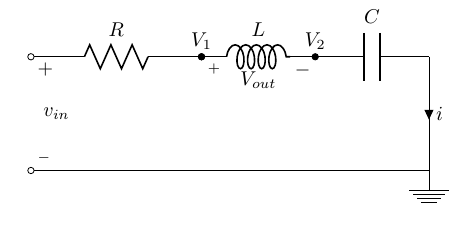
\includegraphics[width=1\linewidth]{img/circuit-RLC}
				\label{fig:circuit-RLC-small}
			\end{figure}
		\end{column}
		
	\end{columns}
	
\end{frame}

\begin{frame}
	
	\frametitle{Example \arabic{exampleCount}: RLC Circuit}
	\begin{itemize}
		\item Writing derivatives of state variables in function of state variables and inputs: 
		$ \left\lbrace  \begin{matrix}
		\frac{di}{dt} = \frac{V_1 - V_2}{L} = \frac{V_{in} - R\cdot i - V_2}{L} \\
		\frac{dV_2}{dt} 
		= \frac{i}{C}	\\
		\end{matrix} 
		\right. 
		$
		\item Writing output in function of state variables and inputs: $V_{out} = V_1 - V_2 = V_{in} - Ri - V_2$
	\end{itemize}
	\begin{block}{State Space Representation}
		This yields the \textbf{State Space Representation} of the dynamic system. In Matrix form:
		\begin{align*}
		\begin{bmatrix}
		\frac{dV_2}{dt} \\
		\frac{di}{dt} \\
		\end{bmatrix} 
		&= 
		\begin{bmatrix}
		0 & 1/C \\
		-1/L & -R/L  \\
		\end{bmatrix} 	
		\begin{bmatrix}
		V_2 \\
		i \\
		\end{bmatrix}
		+ 
		\begin{bmatrix}
		0 \\
		1 \\
		\end{bmatrix}
		V_{in} 
		\\
		V_{out} &= 
		\begin{bmatrix}
		-1 & -R
		\end{bmatrix}
		\begin{bmatrix}
		V_2 \\
		i \\
		\end{bmatrix}
		+ V_{in}
		\end{align*}
	\end{block}	
\end{frame}

\begin{frame}
	\frametitle{Force-Voltage Analogy}
	
	\begin{figure}
		\centering
		\includegraphics[width=0.9\linewidth]{"img/force-voltage"}
		\label{fig:force-voltageanalogy}
	\end{figure}
	
	
	Let:
	\begin{center}
		\begin{tabular*}{0.4\linewidth}{@{\extracolsep{\fill} }c  c @{$\leftrightarrow$} c }
			F	&&	V \\
			$\dot{x}$ && i \\
			x && q \\
		\end{tabular*}
	\end{center}
	
\end{frame}

\begin{frame}
	\frametitle{Force-Voltage Analogy}
	The analogy between the other quantities follows from comparing the physical laws.
	\vspace{2pt}
	\begin{tabular*}{1\linewidth}{@{\extracolsep{\fill}} l l l }
		Damping: & Resistance: & \\
	\end{tabular*}
	\begin{columns}
		\begin{column}{0.25\linewidth}
			\begin{figure}
				\includegraphics[width=1\linewidth]{img/damping}
			\end{figure}
		\end{column}
		
		\begin{column}{0.25\linewidth}
			\hspace{3pt}
			$F = b\dot{x} $ 
		\end{column}
		
		\begin{column}{0.25\linewidth}
			\begin{figure}
				\centering
				\includegraphics[width=1\linewidth]{img/resistor}
				\label{fig:resistor}
			\end{figure}
		\end{column}
		
		\begin{column}{0.25\linewidth}
			\hspace{3pt}
			$V = Ri$
		\end{column}
		
	\end{columns}
	
	\begin{center}
		$\boxed{b \leftrightarrow R} $	
	\end{center}
\end{frame}

\begin{frame}
	\frametitle{Force-Voltage Analogy}
	\begin{columns}
		\begin{column}{0.25\linewidth}
			Spring:
			\begin{figure}
				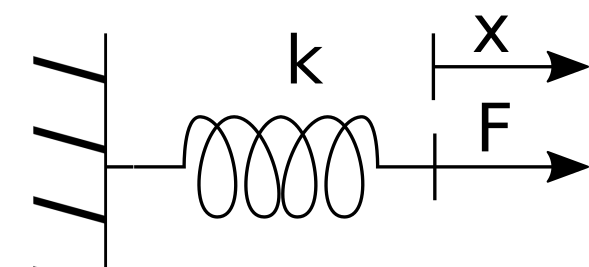
\includegraphics[width=1\linewidth]{img/spring}
			\end{figure}
		\end{column}
		
		\begin{column}{0.25\linewidth}
			\hspace{3pt}
			$F = kx \newline \Rightarrow \frac{dF}{dt} = k\frac{dx}{dt}$ 
		\end{column}
		
		\begin{column}{0.25\linewidth}
			Capacitor:
			\begin{figure}
				\includegraphics[width=1\linewidth]{img/capacitor}
				\label{fig:capacitor}
			\end{figure}
		\end{column}
		
		\begin{column}{0.25\linewidth}
			\hspace{3pt}
			$\frac{dV}{dt} = \frac{i}{C}$
		\end{column}
		
	\end{columns}
	
	\begin{center}
		$\boxed{k \leftrightarrow \frac{1}{C}} $	
	\end{center}
	
	\pause
	
	\begin{columns}
		\begin{column}{0.25\linewidth}
			Newton:
			\begin{figure}
				\includegraphics[width=1\linewidth]{img/newton}
			\end{figure}
		\end{column}
		
		\begin{column}{0.25\linewidth}
			\hspace{3pt}
			\begin{align*}
			F &= m \ddot{x} \\ 
			&= m \frac{d\dot{x}}{dt}
			\end{align*} 
		\end{column}
		
		\begin{column}{0.25\linewidth}
			Coil:
			\begin{figure}
				\includegraphics[width=1\linewidth]{img/coil}
				\label{fig:coil}
			\end{figure}
		\end{column}
		
		\begin{column}{0.25\linewidth}
			\hspace{3pt}
			$V = L\frac{di}{dt}$
		\end{column}
		
	\end{columns}
	
	\begin{center}
		$\boxed{m \leftrightarrow L} $	
	\end{center}
\end{frame}

\begin{frame}
	\stepcounter{exampleCount}
	\frametitle{Example \arabic{exampleCount}: Hoover dam}
	\begin{columns}
		\begin{column}{0.6\linewidth}
			Define:
			\begin{itemize}
				\item Inflow of water: $u(t)$
				\item Current volume of water: $x(t)$
				\item Outflow of water: $y(t)$
				\item Water level: $h(t)$
			\end{itemize}
			Assume that $x(t) = c_1\cdot h(t)$
			
			\vspace{6pt}
			What will happen when we open the gate?
		\end{column}
		\begin{column}{0.4\linewidth}
			\begin{figure}
				\centering
				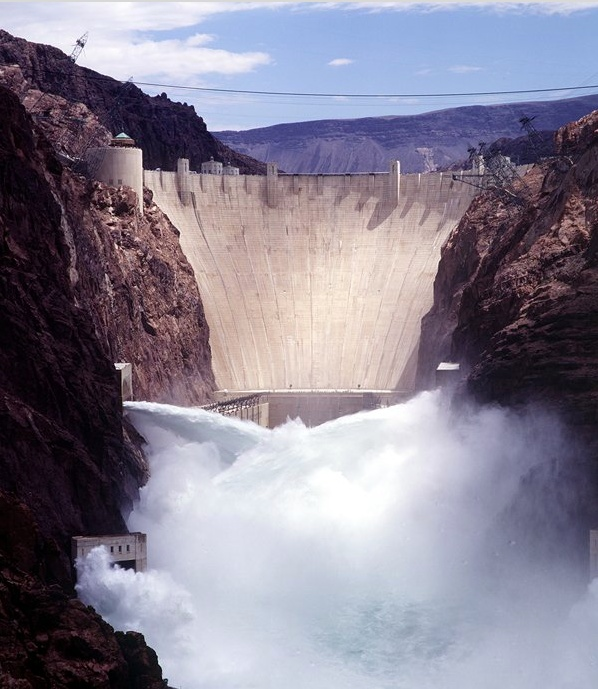
\includegraphics[width=1\linewidth]{img/Hoover-dam}
				\label{fig:Hoover-dam}
			\end{figure}
		\end{column}
	\end{columns}
	
\end{frame}

\begin{frame}
	\frametitle{Example \arabic{exampleCount}: Hoover dam}
	\begin{itemize}
		\item Outflow depends on height: \\
		\hspace{1cm}$y(t) = c_2 \cdot h(t) $
		\item The state of the system is defined by the contained volume of water: \\
		\hspace{1cm}$\dot{x}(t) = u(t) - y(t) = u(t) - c_2\cdot h(t) $
		\item Thus a \textbf{State Space Representation} is, with $c \triangleq \frac{c_2}{c_1}$:
		\begin{align*}
		\dot{x}(t) &= u(t) - c\cdot x(t) \\
		y(t) &= c\cdot x(t) \\
		\end{align*} 
	\end{itemize}
	\vspace{-1cm}
	\begin{center}
		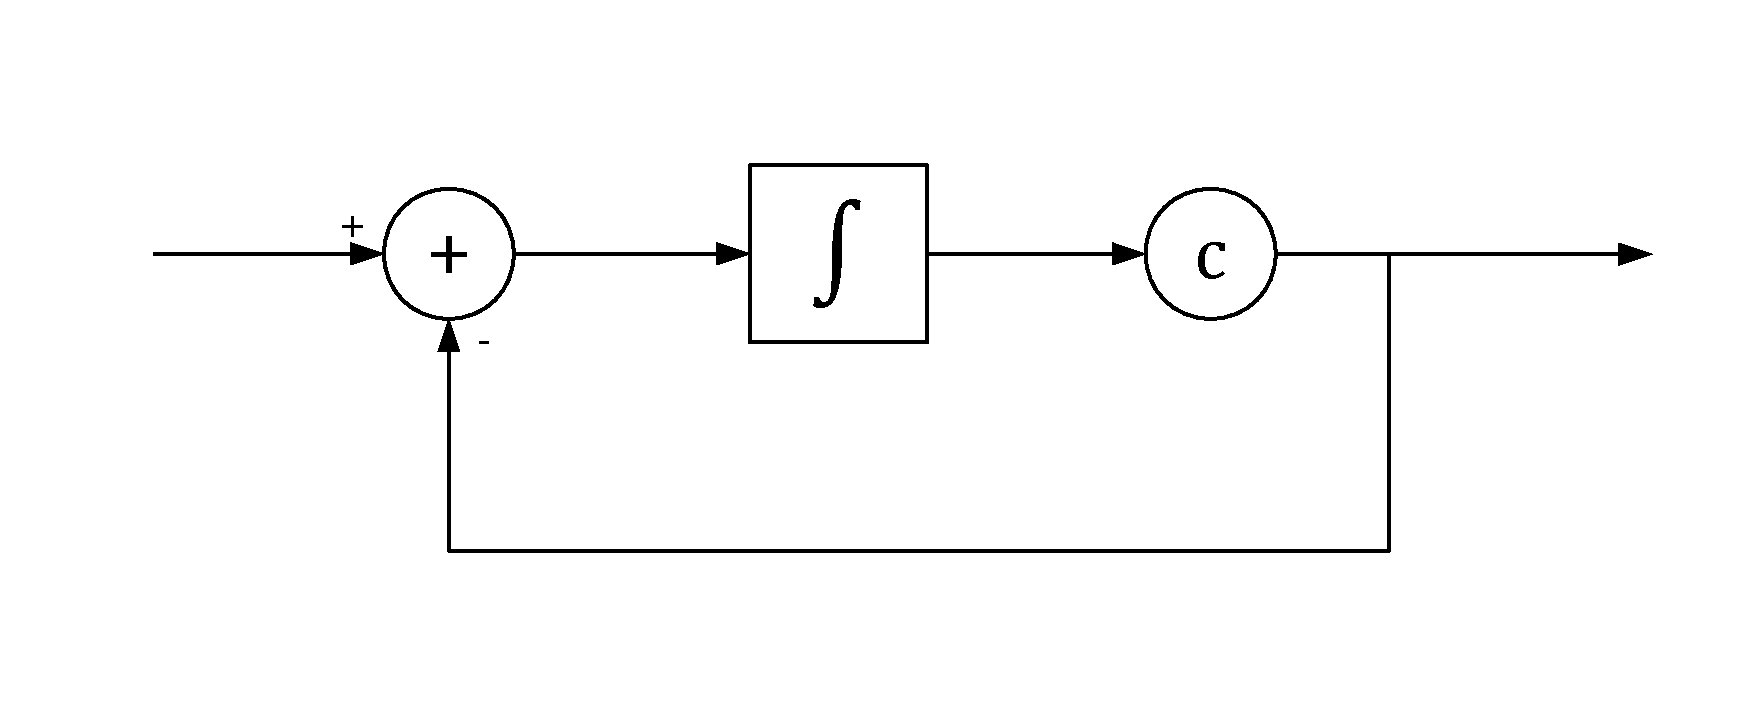
\includegraphics[width=0.75\linewidth]{img/hoover-dam-diagram}
	\end{center}
\end{frame}
